% Options for packages loaded elsewhere
\PassOptionsToPackage{unicode}{hyperref}
\PassOptionsToPackage{hyphens}{url}
\documentclass[
]{article}
\usepackage{xcolor}
\usepackage{amsmath,amssymb}
\setcounter{secnumdepth}{-\maxdimen} % remove section numbering
\usepackage{iftex}
\ifPDFTeX
  \usepackage[T1]{fontenc}
  \usepackage[utf8]{inputenc}
  \usepackage{textcomp} % provide euro and other symbols
\else % if luatex or xetex
  \usepackage{unicode-math} % this also loads fontspec
  \defaultfontfeatures{Scale=MatchLowercase}
  \defaultfontfeatures[\rmfamily]{Ligatures=TeX,Scale=1}
\fi
\usepackage{lmodern}
\ifPDFTeX\else
  % xetex/luatex font selection
\fi
% Use upquote if available, for straight quotes in verbatim environments
\IfFileExists{upquote.sty}{\usepackage{upquote}}{}
\IfFileExists{microtype.sty}{% use microtype if available
  \usepackage[]{microtype}
  \UseMicrotypeSet[protrusion]{basicmath} % disable protrusion for tt fonts
}{}
\makeatletter
\@ifundefined{KOMAClassName}{% if non-KOMA class
  \IfFileExists{parskip.sty}{%
    \usepackage{parskip}
  }{% else
    \setlength{\parindent}{0pt}
    \setlength{\parskip}{6pt plus 2pt minus 1pt}}
}{% if KOMA class
  \KOMAoptions{parskip=half}}
\makeatother
\usepackage{graphicx}
\makeatletter
\newsavebox\pandoc@box
\newcommand*\pandocbounded[1]{% scales image to fit in text height/width
  \sbox\pandoc@box{#1}%
  \Gscale@div\@tempa{\textheight}{\dimexpr\ht\pandoc@box+\dp\pandoc@box\relax}%
  \Gscale@div\@tempb{\linewidth}{\wd\pandoc@box}%
  \ifdim\@tempb\p@<\@tempa\p@\let\@tempa\@tempb\fi% select the smaller of both
  \ifdim\@tempa\p@<\p@\scalebox{\@tempa}{\usebox\pandoc@box}%
  \else\usebox{\pandoc@box}%
  \fi%
}
% Set default figure placement to htbp
\def\fps@figure{htbp}
\makeatother
\setlength{\emergencystretch}{3em} % prevent overfull lines
\providecommand{\tightlist}{%
  \setlength{\itemsep}{0pt}\setlength{\parskip}{0pt}}
\usepackage{bookmark}
\IfFileExists{xurl.sty}{\usepackage{xurl}}{} % add URL line breaks if available
\urlstyle{same}
\hypersetup{
  hidelinks,
  pdfcreator={LaTeX via pandoc}}

\author{}
\date{}

\begin{document}

\section{Paper 10: Emergent Gauge
Structure}\label{paper-10-emergent-gauge-structure}

\subsection{Kinematic Uniqueness of the Connection, the First Holonomy,
the Forcing of the Structure Group SO(4), the Spin Lift, and the
Kinematic Default of the Coupling
Constant}\label{kinematic-uniqueness-of-the-connection-the-first-holonomy-the-forcing-of-the-structure-group-so4-the-spin-lift-and-the-kinematic-default-of-the-coupling-constant}

Author: Noriaki Kihara\\
Affiliation: WF System Co., Ltd.\\
ORCID: 0009-0004-6753-4020\\
Version: v0.2\\
Date: June 2026\\
DOI (this version): 10.5281/zenodo.20640465\\
Concept DOI: 10.5281/zenodo.20640464\\
License: CC BY 4.0

\begin{center}\rule{0.5\linewidth}{0.5pt}\end{center}

\subsection{Abstract}\label{abstract}

This paper shows that the kinematic skeleton of gauge theory appears
inside the reciprocal dual model (Papers 1--9) \textbf{without ever
assuming the gauge principle}. The direction of approach is the reverse
of the usual one: each time we pressed on different questions --- the
inventory of conserved quantities, stability, and observability ---
components of gauge theory appeared as by-products.

The main results are as follows. (1) \textbf{Kinematic uniqueness of the
connection}: the radial direction of each fragment is the indicator of
its local timelike axis (Paper 6), and the connection must transport it.
The two conditions of time-axis transport and twist-free minimality
uniquely select the minimal-rotation connection of the position-adapted
frame --- no dynamical input was required. (2) \textbf{The first
holonomy}: the sibling-triangle holonomy of a mutually orthogonal
three-fragment configuration (tripod) is a \(90^\circ\) rotation, and
its rotation angle \textbf{coincides exactly} with the area of the
geodesic triangle on the direction sphere (an octant, \(\pi/2\)) ---
discrete transport reproduces continuous curvature exactly. The
curvature quantum \(\pi/2\) is universal, independent of shell and
hierarchy. The second exact holonomy \(\arccos(4/5)\) has infinite order
by Niven's theorem, so the holonomy group is infinite. (3)
\textbf{Continuization theorem for the structure group}: the closure of
the group generated by adjoining to \(B_4\) the \(45^\circ\) rotation
required by transport between fragments of different shapes is all of
SO(4) (proved via the 3-dimensional crystallographic restriction).
\textbf{The continuous gauge group is a consequence, not an assumption.}
(4) \textbf{The locus of curvature}: curvature on genealogical links and
static transverse twist are unrecordable and hence gauge (a derivation
from the record theorem). Curvature concentrates on sibling triangles,
and the place where internal gauge structure can be physical is
localized at transition events (vertices). (5) \textbf{Spin lift}: the
half-angle lift is consistent; the tripod holonomy has order 8 in the
spin representation, and the all-axes planar ring configuration carries
the first loop that is trivial in the vector representation and \(-1\)
in the spin representation. The screw lift (coupling rotation with
translation) is unique with pitch \(1/2\) and identifies a new
gauge-invariant \(Z_2\), the excitation parity \((-1)^{\Sigma|k|}\). (6)
\textbf{Kinematic default of the coupling constant}: for the parameter
\(\beta\) of Wilson-type weights, we show that pure counting
(\(\beta=0\)) is forced under the current axiom system --- a finite
\(\beta\) would signify genuinely new dynamical input.

Finally, we identify the gauge structure that has emerged as being not
of Yang--Mills type but of the type of \textbf{first-order gravity
(vierbein plus spin connection)}. The claim of this paper extends only
to ``gauge structure plus computed holonomies''; we do not claim a
``gauge theory.''

\begin{center}\rule{0.5\linewidth}{0.5pt}\end{center}

\subsection{Keywords}\label{keywords}

lattice gauge theory, connection, holonomy, parallel transport,
hyperoctahedral group, crystallographic restriction, spin structure,
double cover, Wilson action, vierbein

\begin{center}\rule{0.5\linewidth}{0.5pt}\end{center}

\subsection{1. Introduction}\label{introduction}

Gauge theory on a lattice has been established since Wilson {[}5{]} as a
construction that places continuous gauge groups on a discrete spacetime
(see Kogut {[}6{]} for a review). The construction of this paper runs in
the opposite direction: \textbf{the discrete structure (a
\(B_4\)-symmetric lattice and configuration statistics) comes first, and
the continuous group is forced}. Moreover, whereas ordinary gauge theory
{[}7{]} starts from localizing an internal symmetry, what emerges in
this paper is the transport rule for the orthonormal frame of each
fragment --- an object close to the first-order formulation of gravity
(Cartan's frame formalism). The tradition of treating curvature in
discrete geometry goes back to Regge {[}8{]}.

The question of this paper is modest: when the multi-fragment
configurations constructed in Paper 7 are endowed with the structure of
frame alignment \textbf{by minimal choices}, what becomes determined and
what remains free?

\begin{center}\rule{0.5\linewidth}{0.5pt}\end{center}

\subsection{2. Setup: Graph, Frames, and
Links}\label{setup-graph-frames-and-links}

Following the splitting representation of Paper 4 {[}1{]}, for a single
splitting event \(9\to(s_A,s_B,s_C)\) we take: nodes = the parent and
the children (each carrying the orthonormal 4-frame of its own internal
lattice), links = genealogical links and sibling links, minimal cycles =
sibling triangles. A child \(X\) occupies cell \(k_X\) of the parent
lattice (configuration reading, Paper 7 {[}3{]}).

There are two candidate frame conventions: (L) all children inherit the
parent's lattice frame (all links identity, all holonomies trivial); (A)
the first frame vector of each child = its own cell direction
\(\hat k_X\) (position-adapted).

\begin{center}\rule{0.5\linewidth}{0.5pt}\end{center}

\subsection{3. Kinematic Uniqueness of the
Connection}\label{kinematic-uniqueness-of-the-connection}

\subsubsection{3.1 Time-axis transport
condition}\label{time-axis-transport-condition}

By Paper 6 {[}2{]}, the manifestation of the asymmetric bit within a
hierarchy concentrates in the radial direction --- the radial direction
\(\hat k_X\) of each fragment is the indicator of that fragment's
\textbf{local timelike axis}. A necessary condition for the connection
to be compatible with this structure is that the link variable map
radial direction to radial direction: \(U_{AB}(\hat k_A)=\hat k_B\). The
lattice convention (L) maps A's timelike axis to a spacelike direction
of B whenever \(\hat k_A\ne\hat k_B\), which is incompatible with the
hierarchical universality of the \(1{+}3\) decomposition. \textbf{Hence
(L) is excluded.}

\subsubsection{3.2 Uniqueness theorem}\label{uniqueness-theorem}

If, on the transverse freedom remaining under the time-axis transport
condition, we impose the \textbf{twist-free condition} (identity on the
orthogonal complement of the plane spanned by the two directions =
minimal rotation), then:

\begin{quote}
\textbf{Theorem}: A connection satisfying time-axis transport and
twist-freeness coincides uniquely with the minimal-rotation connection
of the position-adapted convention. No dynamical input is required.
\end{quote}

For a non-antipodal pair of axis-type directions the minimal rotation is
a unique \(90^\circ\) rotation, an element of \(B_4\).

\begin{center}\rule{0.5\linewidth}{0.5pt}\end{center}

\subsection{4. Holonomy}\label{holonomy}

\subsubsection{4.1 The first holonomy: the tripod carries a quarter
turn}\label{the-first-holonomy-the-tripod-carries-a-quarter-turn}

The holonomy of the sibling triangle \(e_1\to e_2\to e_3\to e_1\) of a
mutually orthogonal configuration \(\{e_1,e_2,e_3\}\) (the tripod class
of Paper 7) is

\[
H=\text{a }90^\circ\text{ rotation in the }(e_2,e_3)\text{ plane (nontrivial, order 4, }\det=+1\text{)}
\]

(the matrix computation is in the Appendix). The geodesic triangle
\((e_1,e_2,e_3)\) on the direction sphere has three right angles and
area \(=\tfrac{3\pi}2-\pi=\tfrac\pi2\). \textbf{Holonomy angle = area}:
discrete transport (the minimal rotations of \(B_4\)) reproduces
continuous curvature (Gauss--Bonnet) exactly. The curvature quantum
\(\pi/2\) of the orthogonal tripod is independent of shell, hierarchy,
and shape, so long as the directions are mutually orthogonal --- a
scale-invariant curvature quantum.

\begin{figure}
\centering
\pandocbounded{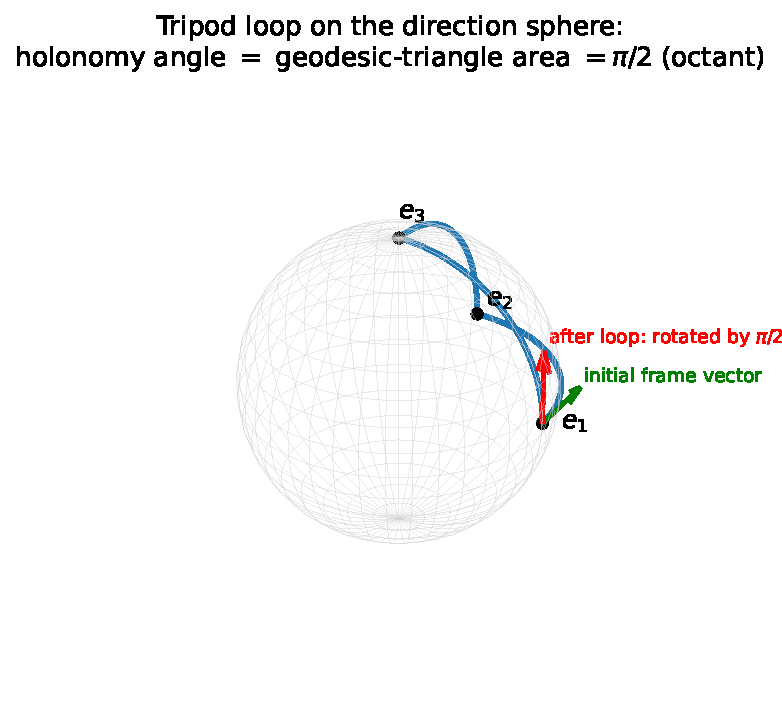
\includegraphics[keepaspectratio,alt={Figure 1. Tripod-loop holonomy equals the geodesic-triangle area}]{figure_paper10_1_tripod_holonomy.pdf}}
\caption{Figure 1. Tripod-loop holonomy equals the geodesic-triangle
area}
\end{figure}

\textbf{Figure 1. Tripod-loop holonomy: the geodesic triangle on the
direction sphere (an octant, three right angles). The transported frame
vector rotates by \(\pi/2\) around one circuit = the triangle area (an
exact discrete reproduction of Gauss--Bonnet).}

\subsubsection{4.2 Relational resolution of the antipodal
ambiguity}\label{relational-resolution-of-the-antipodal-ambiguity}

In the antipodal-pair class the transport \(e_1\to-e_1\) requires a
choice of plane for the \(180^\circ\) rotation and is not unique. If it
is defined by geodesic composition via the remaining sibling (the
relational rule: no reference imported from outside), the holonomy in
the vector representation trivializes canonically. The difference
between area \(0\) and area \(2\pi\) is invisible in the vector
representation and becomes visible only with the spin lift (§6).

\subsubsection{4.3 The second exact holonomy and
infiniteness}\label{the-second-exact-holonomy-and-infiniteness}

For the configuration \((2,1,0,0)/\sqrt5,\ (1,2,0,0)/\sqrt5,\ e_3\), the
holonomy angle of the geodesic triangle is, by spherical excess,
\(\arccos(4/5)\approx36.87^\circ\). By Niven's theorem {[}9{]} (if
\(\cos\theta\in\mathbb{Q}\) and \(\theta/\pi\in\mathbb{Q}\), then
\(\cos\theta\in\{0,\pm\tfrac12,\pm1\}\)), \(\arccos(4/5)/\pi\) is
irrational, so this holonomy has \textbf{infinite order}. The holonomy
group is infinite, and the continuization of the structure group (§5)
manifests at the level of observables.

\begin{figure}
\centering
\pandocbounded{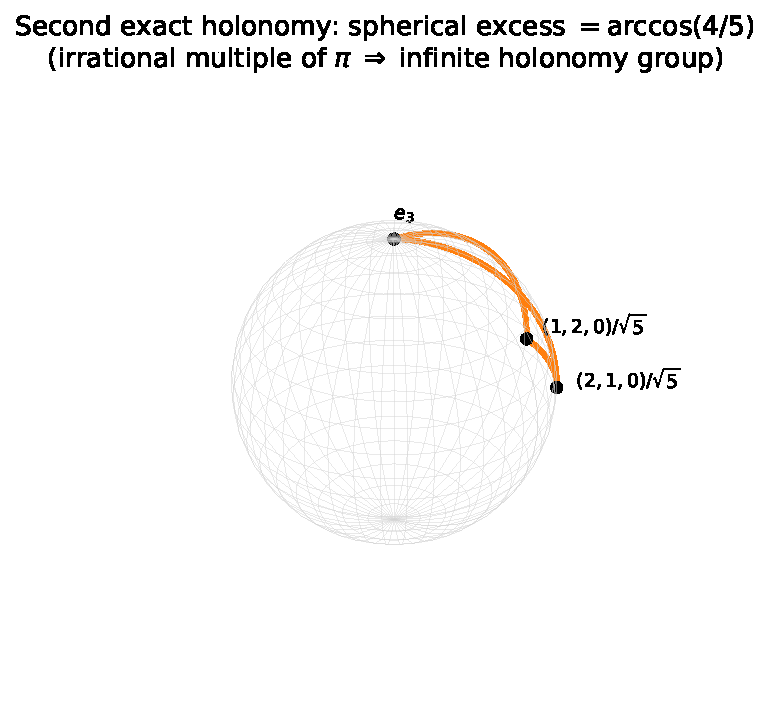
\includegraphics[keepaspectratio,alt={Figure 2. Second exact holonomy: infinite holonomy group}]{figure_paper10_2_holonomy_arccos45.pdf}}
\caption{Figure 2. Second exact holonomy: infinite holonomy group}
\end{figure}

\textbf{Figure 2. The second exact holonomy: the spherical excess of a
configuration of type \(((2,1,0,0),(1,2,0,0),e_3)/\sqrt5\) is
\(\arccos(4/5)\) --- an irrational multiple of \(\pi\) (Niven's
theorem), so the holonomy group is infinite.}

\subsubsection{4.4 The locus of curvature (a derivation from the record
theorem)}\label{the-locus-of-curvature-a-derivation-from-the-record-theorem}

Even if curvature is placed on a genealogical link, no record exists at
any hierarchy level that reads the relative frames of the cousins where
its effect would have to appear (half-wavelength censorship, Paper 9
{[}4{]}). Since a difference that is not recorded has no fact (the
record theorem, Paper 6):

\begin{quote}
\textbf{Theorem}: Genealogical curvature and static transverse twist are
gauge. The physical locus of curvature is restricted to sibling
triangles (star-flatness is not a convention but a canonical gauge), and
the holonomy of any genealogical cycle decomposes into an ordered
product of sibling-triangle holonomies (a discrete non-abelian Stokes).
The place where internal gauge structure can be physical is localized
not at links but at \textbf{transition events (vertices)}.
\end{quote}

\begin{center}\rule{0.5\linewidth}{0.5pt}\end{center}

\subsection{5. Continuization Theorem for the Structure
Group}\label{continuization-theorem-for-the-structure-group}

\subsubsection{5.1 The obstruction}\label{the-obstruction}

Position adaptation requires \(U_{AB}(\hat k_A)=\hat k_B\), but \(B_4\)
(components \(\{0,\pm1\}\)) maps axis-type directions only to axis-type
directions. Since the cell directions of shell 5 are of diagonal type
(\((\pm e_i\pm e_j)/\sqrt2\)), \textbf{no \(B_4\)-valued link variable
exists on links between fragments of different shapes} (the required
\(45^\circ\) rotation contains components \(\pm1/\sqrt2\)).

\subsubsection{5.2 Theorem}\label{theorem}

\begin{quote}
\textbf{Theorem (continuization)}: The closure of the group generated by
adjoining to \(B_4\) the \(45^\circ\) rotation in a coordinate plane
required by hetero-shape links is all of SO(4).
\end{quote}

\textbf{Sketch of proof}: There is no finite 3-dimensional point group
containing order-8 rotations about two distinct axes (the
crystallographic restriction). Hence the generated group is infinite,
and its closure reaches SO(4) through a family of SO(3) subgroups.
Finite extensions (e.g., \(W(F_4)\)) have also been checked to be
insufficient, by the lengthwise conservation of orbits. \(\blacksquare\)

\begin{quote}
\textbf{The continuous gauge group is a consequence, not an assumption.}
The target picture is ``a structure on a discrete lattice carrying an
SO(4)-valued connection, whose finite remnant is \(B_4\),'' which is
isomorphic to the standard picture of lattice gauge theory {[}5,6{]}.
\end{quote}

\begin{center}\rule{0.5\linewidth}{0.5pt}\end{center}

\subsection{6. Spin Lift}\label{spin-lift}

\subsubsection{6.1 Construction and
consistency}\label{construction-and-consistency}

Each minimal rotation (of angle \(\theta\)) is lifted to
\(\mathrm{Spin}(4)\) by the half-angle lift \(\exp(\tfrac\theta2 B)\).
Since antipodal transport lifts as the composition prescribed by the
relational rule (§4.2), its sign is fixed and the lift is consistent. A
quaternion computation shows that the lift of the tripod holonomy is
\(H_{\mathrm{spin}}=(1+i)/\sqrt2\), with \(H_{\mathrm{spin}}^4=-1\):
\textbf{a spinor carried four times around the tripod triangle reverses
sign} (invisible in the vector representation).

\subsubsection{\texorpdfstring{6.2 The first
\(-1\)}{6.2 The first -1}}\label{the-first--1}

The great-circle 4-cycle of the all-axes planar ring configuration
\(\{e_1,e_2,-e_1,-e_2\}\) is the identity in the vector representation
and \(-1\) in the spin representation --- \textbf{the first loop that is
vectorially trivial and spinorially nontrivial}. The enclosed area is a
hemisphere, \(2\pi\); the sign is \((-1)^{\text{area}/2\pi}\), and a
\(Z_2\) degree of loops is born. Moreover, the lift of the exchange of
like fragments gives exchange\(^2=-1\) (raw material for spin
statistics; the spinorial matter that would bridge them is not
constructed in this paper).

\subsubsection{6.3 The screw lift and excitation
parity}\label{the-screw-lift-and-excitation-parity}

The current real standing-wave dictionary transforms by whole angles
(vectorially) under rotational transport and contains no matter that
detects \(-1\) (by the general lemma that amplitude-free matter is a
permutation representation, hence single-valued). The half-angle
structure lies on the translation side: the only translation that acts
as a scalar (\(\pm1\)) on each cell of the real dictionary is the
half-period translation (\textbf{the pitch-\(1/2\) uniqueness theorem}),
and the \textbf{screw lift}, which couples a translation to each
rotation, can be defined uniquely in the lattice-plane sector. The
structure group is the direct product \(\mathrm{SO}(4)\times T^4\)
(because under the Euclidean composition the translations would cancel
around closed cycles), and the translation components behave as internal
\(U(1)^4\) charges subordinate to the rotations. The screw outcome of a
\(2\pi\) planar rotation acts on cell \(k\) as \((-1)^{|k_i|+|k_j|}\),
identifying a new gauge-invariant parity

\[
\varepsilon(k)=(-1)^{\sum_i|k_i|}
\]

(finer than shells: both parities can coexist within the same shell). We
also place on record that the combination of two-valued logical states,
\(Z_2\) structure, and protection by censorship is structurally adjacent
to the correspondence between error-correcting codes and \(Z_2\) lattice
gauge theory (Kitaev's toric code {[}10{]}). The \textbf{necessity of
introducing} the screw lift is explicitly left undecided in this paper.

\begin{figure}
\centering
\pandocbounded{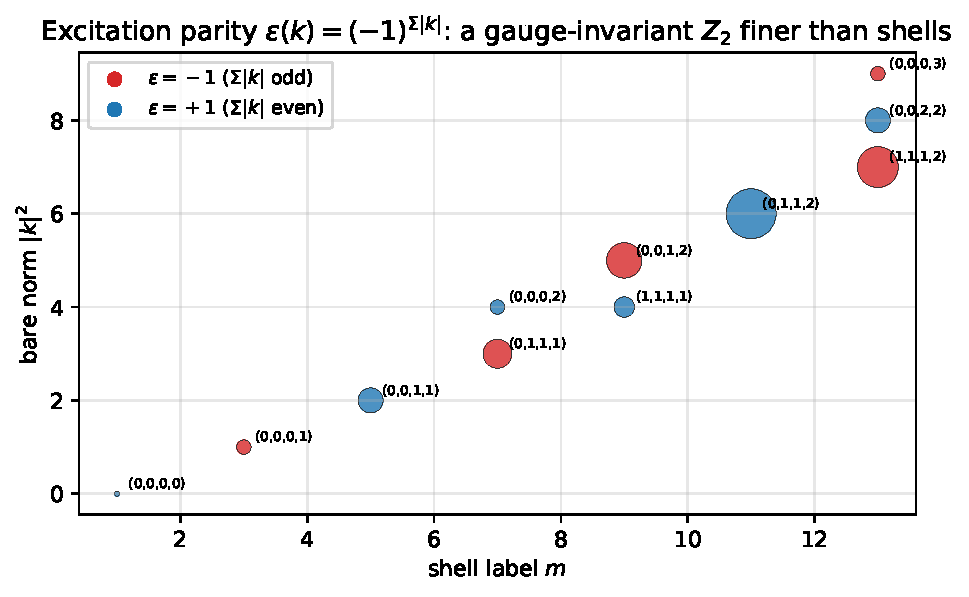
\includegraphics[keepaspectratio,alt={Figure 3. Excitation parity: a gauge-invariant Z2 finer than shells}]{figure_paper10_3_excitation_parity.pdf}}
\caption{Figure 3. Excitation parity: a gauge-invariant Z2 finer than
shells}
\end{figure}

\textbf{Figure 3. Excitation parity
\(\varepsilon(k)=(-1)^{\Sigma|k_i|}\) (exhaustive for \(m\le13\)): point
size = number of cells in the orbit, color = parity. Both parities
coexist within the same shell --- a gauge-invariant \(Z_2\) finer than
shells.}

\begin{center}\rule{0.5\linewidth}{0.5pt}\end{center}

\subsection{7. Kinematic Default of the Coupling
Constant}\label{kinematic-default-of-the-coupling-constant}

Consider a Wilson-type action {[}5{]} with
\(s(H)=1-\tfrac14\mathrm{Tr}\,H\) per sibling triangle and weight
\(\propto e^{-\beta s}\); then only tripods carry \(s=\tfrac12\), and
the branching ratios (Paper 7) are deformed into a one-parameter family.
However:

\begin{enumerate}
\def\labelenumi{\arabic{enumi}.}
\tightlist
\item
  Frame frustration (the unsatisfiability of global alignment at
  tripods) does not separate the configuration pair (tripod and
  antipodal pair) that is exactly degenerate in capacity, energy, and
  fragment content --- \textbf{it posts no debit in the area ledger}
  (kinematically free).
\item
  The counting of vertex variables (the initialization of child frames
  at splitting events) yields only the two values \(\beta=0\) for
  relaxed alignment and \(\beta=\infty\) for exact alignment.
\end{enumerate}

\begin{quote}
\textbf{Theorem (kinematic default)}: Under the current axiom system
(the three assumptions + configuration reading + the record principle),
the weight of the branching ratios is forced to be pure counting
(\(\beta=0\)). A finite \(\beta\) would signify the existence of
genuinely new dynamical input, and a branching-ratio measurement (12.9\%
/ 0\% / intermediate values) becomes a three-way discriminator. The
difference that the choice of measure (batch / sequential / path) makes
to the branching statistics is treated in Paper 12 §5.3.
\end{quote}

\begin{center}\rule{0.5\linewidth}{0.5pt}\end{center}

\subsection{8. Identification and the Discipline of
Naming}\label{identification-and-the-discipline-of-naming}

The precise counterpart of the structure that has emerged is not the
Yang--Mills theory of internal symmetries {[}7{]}: the position-adapted
frames = a discrete frame field (vierbein), the connection = a spin
connection, the structure group SO(4) = the rotation group of the
tangent space. That is, it is close to \textbf{the gauge structure of
first-order gravity} (a structural correspondence, not an
identification).

The claim of this paper extends only to ``gauge structure plus computed
holonomies.'' What is missing for claiming a ``gauge theory'' ---
propagating gauge degrees of freedom, dynamics of an action, spinorial
matter, internal symmetries --- is explicitly placed outside the scope
of claims.

\begin{center}\rule{0.5\linewidth}{0.5pt}\end{center}

\subsection{9. Scope of Claims of This
Paper}\label{scope-of-claims-of-this-paper}

What we claim: (1) Kinematic uniqueness of the connection (theorem). (2)
Holonomy \(\pi/2\) = geodesic area (exact), the infinite order of
\(\arccos(4/5)\) (Niven), the infiniteness of the holonomy group. (3)
The continuization theorem (the forcing of SO(4)). (4) The gauge nature
of genealogical curvature and static twist, and the concentration of
curvature on sibling triangles (a derivation from the record theorem).
(5) The consistency of the spin lift, order 8, the first \(-1\), the
uniqueness of pitch \(1/2\), the excitation parity \(\varepsilon\). (6)
The kinematic forcing of \(\beta=0\).

What we do not claim: (1) Correspondence with the gauge groups,
representations, or generation structure of the Standard Model. (2)
Dynamics of gauge fields (propagation, scattering). (3) The existence of
fermions (exchange\(^2=-1\) is raw material; spinorial matter is not
constructed). (4) The necessity of the screw lift. (5) The title of
``gauge theory.''

\begin{center}\rule{0.5\linewidth}{0.5pt}\end{center}

\subsection{10. Conclusion}\label{conclusion}

Without placing the gauge principle among the axioms, the connection,
curvature, a continuous structure group, spin structure, and even the
default value of the coupling constant have emerged as by-products of
questions about stability and observability. In particular, the three
points --- (i) the connection is fixed uniquely by kinematics without
waiting for dynamics, (ii) the holonomy of discrete transport reproduces
continuous curvature exactly, and (iii) the continuous group is
\textbf{forced} by the crystallographic restriction --- provide an
independent instance of the picture of continuous gauge structure on top
of a discrete foundation. The remaining open items --- internal gauge
fields localized at vertices, spinorial matter, finite coupling --- all
converge on a single object: the structure of transition events (the
vertex map).

\begin{center}\rule{0.5\linewidth}{0.5pt}\end{center}

\subsection{Appendix: Matrices and
Verifications}\label{appendix-matrices-and-verifications}

This appendix contains the explicit matrices of the \(90^\circ\)
rotations \(U_{12},U_{23},U_{31}\) and the verification of the holonomy
\(H=U_{31}U_{23}U_{12}\) (\(e_1\to e_1\), \(e_2\to e_3\),
\(e_3\to-e_2\), \(H^4=\mathbf{1}\)), the spin lift by quaternions
(\(q_3q_2q_1=(1+i)/\sqrt2\)), the one-line proof of the obstruction
theorem (the contradiction between the \(B_4\) components \(\{0,\pm1\}\)
and \(1/\sqrt2\)), and the proof of pitch uniqueness
(\(2\pi t\in\{0,\pi\}\bmod 2\pi\)). All of these are exact algebra by
hand; the scripts and research notes are provided in the public
repository (https://github.com/WurabeSeiji/ai-chat-logs-open).

\begin{center}\rule{0.5\linewidth}{0.5pt}\end{center}

\subsection{References}\label{references}

{[}1{]} Noriaki Kihara, Paper 4, v1.0, 2026. Concept DOI:
10.5281/zenodo.20638962.

{[}2{]} Noriaki Kihara, Paper 6, v0.2, 2026. Concept DOI: 10.5281/zenodo.20640456.

{[}3{]} Noriaki Kihara, Paper 7, v0.2, 2026. Concept DOI: 10.5281/zenodo.20640458.

{[}4{]} Noriaki Kihara, Paper 9, v0.2, 2026. Concept DOI: 10.5281/zenodo.20640462.

{[}5{]} K. G. Wilson, ``Confinement of quarks,'' Physical Review D 10
(1974), 2445--2459.

{[}6{]} J. B. Kogut, ``An introduction to lattice gauge theory and spin
systems,'' Reviews of Modern Physics 51 (1979), 659--713.

{[}7{]} C. N. Yang and R. L. Mills, ``Conservation of isotopic spin and
isotopic gauge invariance,'' Physical Review 96 (1954), 191--195.

{[}8{]} T. Regge, ``General relativity without coordinates,'' Il Nuovo
Cimento 19 (1961), 558--571.

{[}9{]} I. Niven, \emph{Irrational Numbers}, Mathematical Association of
America, 1956.

{[}10{]} A. Kitaev, ``Fault-tolerant quantum computation by anyons,''
Annals of Physics 303 (2003), 2--30.

\begin{center}\rule{0.5\linewidth}{0.5pt}\end{center}

\subsection{License}\label{license}

This paper is published under CC BY 4.0.\\
Reuse, adaptation, translation, and citation are permitted, provided
that the author name, version, publication date, and source are clearly
indicated.

\end{document}
